\documentclass[12pt]{beamer}
 
\usepackage[utf8]{inputenc}
\usepackage{tikz}
\usepackage[mathscr]{euscript}

\usetheme{Madrid}
\usecolortheme{beaver}
 
%Information to be included in the title page:
\title[Category Theory]{A first introduction to category theory}
\author[Quinn Murphey]{Quinn Murphey}
\date[]{May 9, 2019}

%Presentation Topics
%
% What is category/purpose
% Define Set and Class
% Define Morphism
% Define Category
% 
% 
% 
% 

\begin{document}
 
\frame{\titlepage}

\begin{frame}{Introduction}
    \frametitle{Introduction}
    \textbf{Main Questions:}
    \begin{itemize}
        \item Why do we care about category theory?
        \item What is category theory?
        \item How can category be utilized?
    \end{itemize}
\end{frame}

\begin{frame}{Why?}
    \frametitle{Why do we care about category theory}
    \begin{itemize}
        \item Provides an alternative formal language than that of set theory.
        \item Allows for generalization of theorems across all of mathematics.
        \item Most importantly, provides a different perspective on mathematical structures.
    \end{itemize}
\end{frame}

\begin{frame}{ZFC vs Category of Sets}
    \center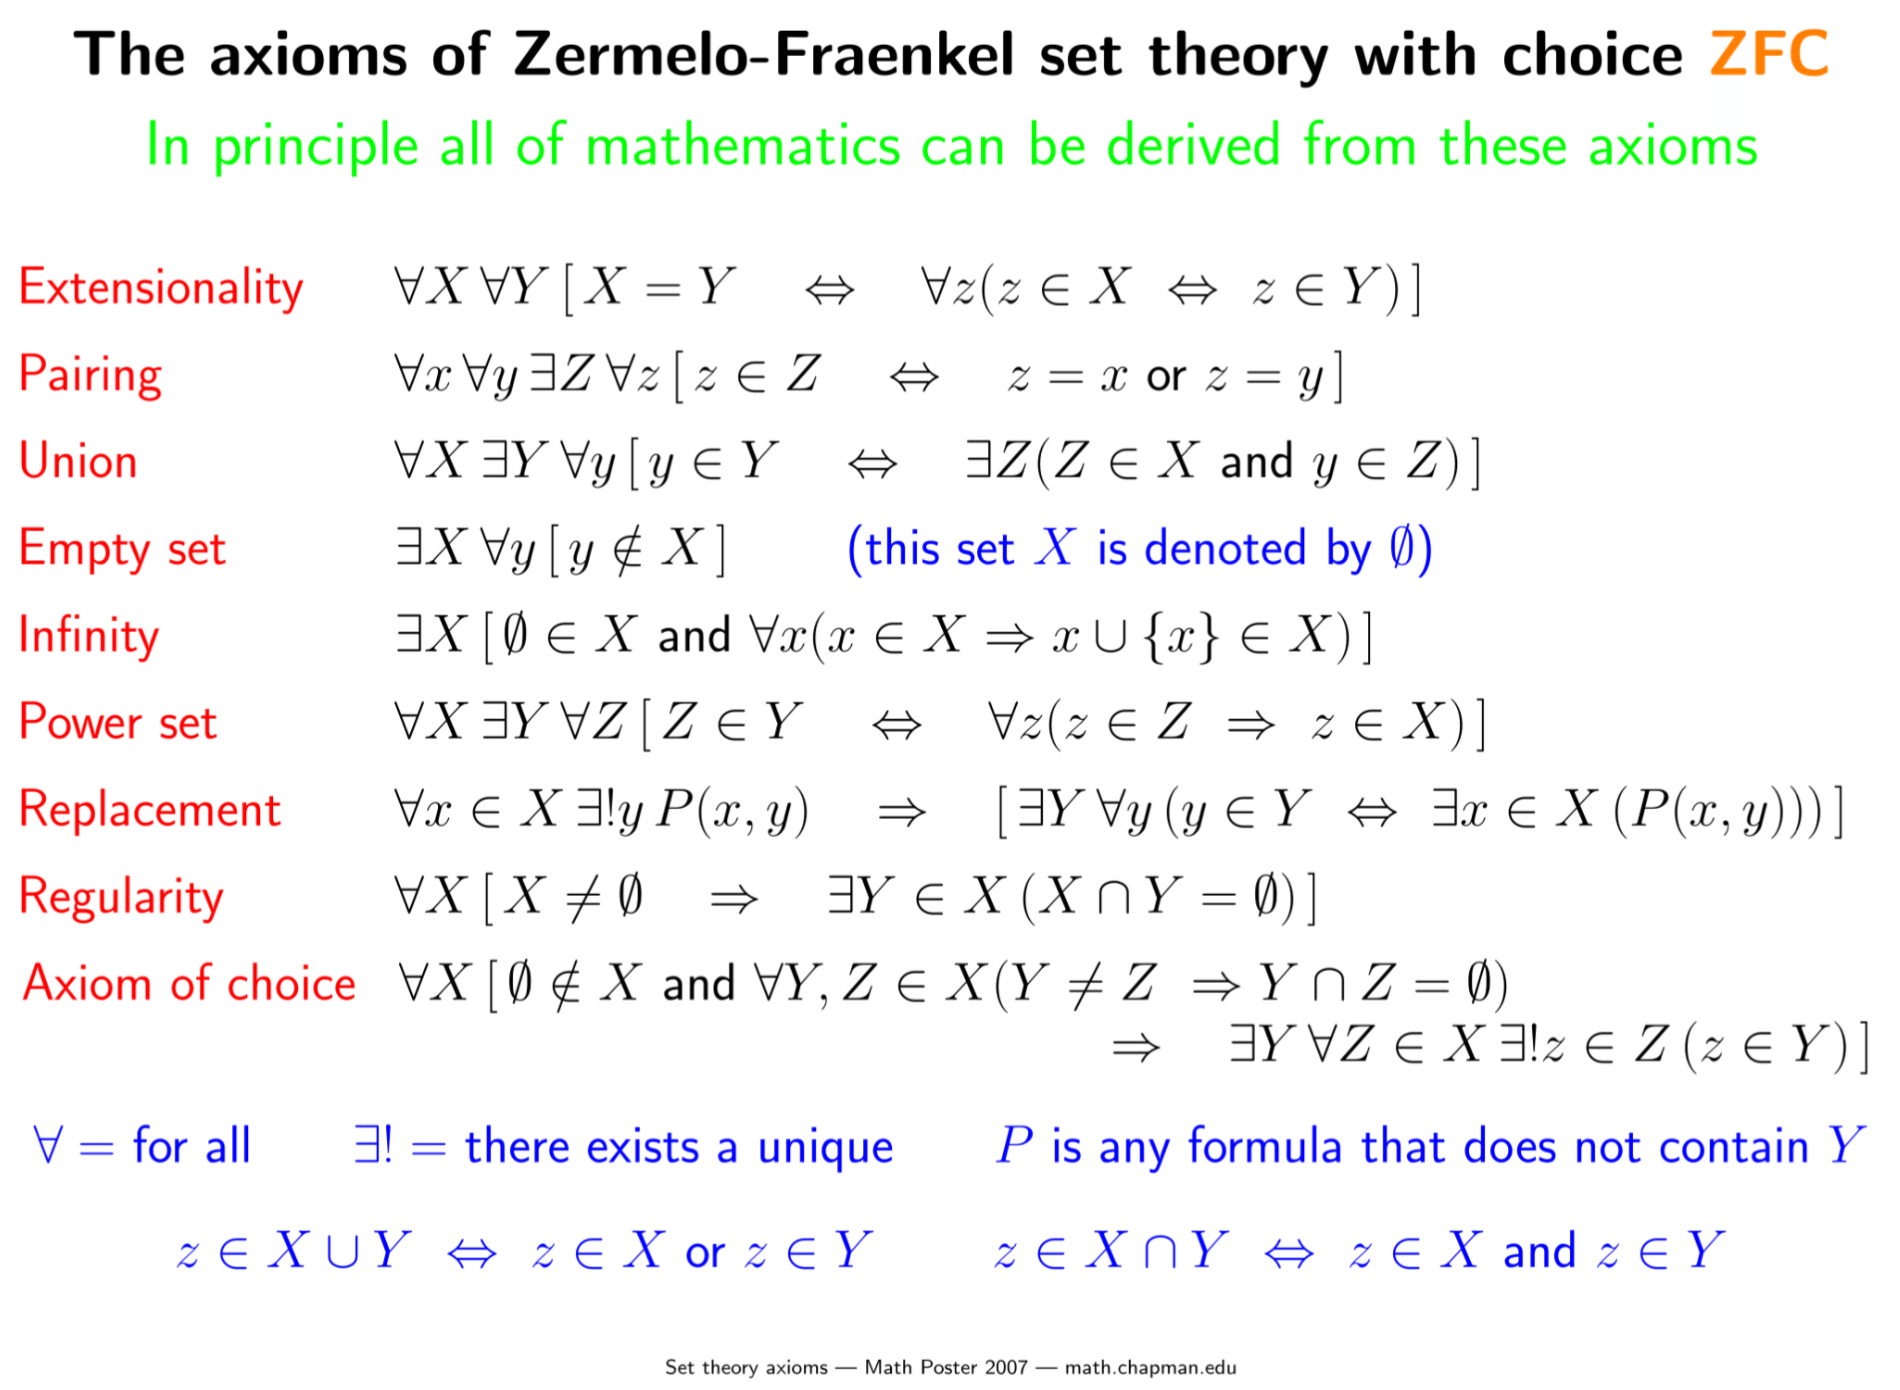
\includegraphics[width=.8\linewidth]{Presentations/ZFC.png}
\end{frame}

\begin{frame}{ZFC vs Category of Sets}
    The axioms of the category of sets
    \center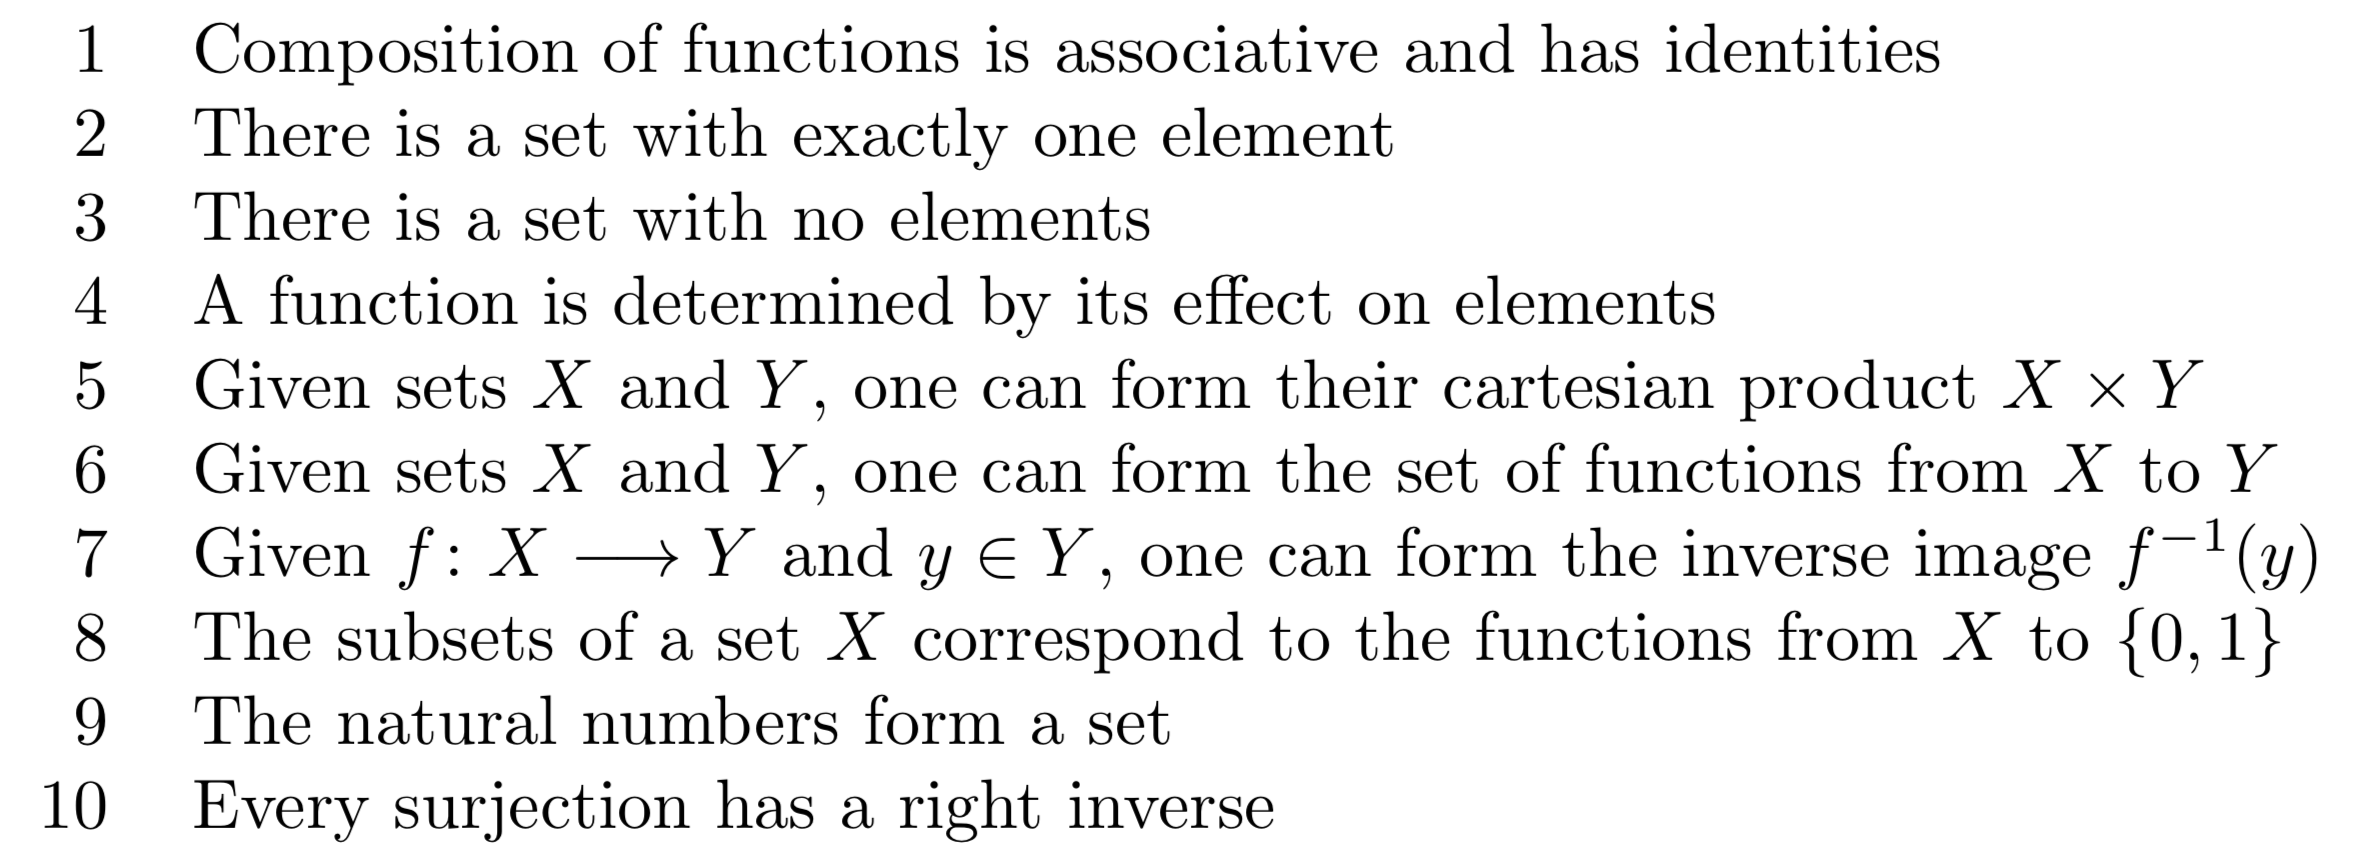
\includegraphics[width=\linewidth]{Presentations/CoS.png}
\end{frame}

\begin{frame}{Definitions}
    
    \begin{block}{Definition: Class}
        A collection of objects that can be unambiguously defined by a property that all its members share.
    \end{block}
    
    \begin{block}{Definition: Set}
        A class which satisfies the ZFC axioms.
    \end{block}
    
    \begin{block}{Definition: Morphism}
        An object $f$ with a source $A$ and a target $B$ denoted $f:A\rightarrow B$ along with a binary operation ``Composition'' which is associative and identity morphisms exists.
    \end{block}
    
\end{frame}

\begin{frame}{Definition: Category}
    A category $\mathscr{C}$ is a class of objects $A,B,C,\dots$ together with a class of disjoint sets denoted hom$(A,B)$ pairwise for each object in $\mathscr{C}$.
    \begin{itemize}
        \item Each set $\hom(A,B)$'s elements $f,g,h,\dots$ are morphisms and written $f:A\rightarrow B$ and likewise. 
        \begin{itemize}
            \item Each composition of morphisms in $\hom(A,B)$ is a morphism in $\hom(A,B)$.
            \item Each $\hom(A,B)$ has two identity morphisms: The right identity $1_A$ and the left identity $1_B$.
        \end{itemize}
    \end{itemize}
\end{frame}

\begin{frame}{Example 1: The Category of Sets}
    Let $\mathscr{S}$ be the category such that each object $A,B,C\dots\in\mathscr{S}$ is a set and every morphism is a function. We call $\mathcal{G}$ the category of sets.
    
    \quad
    
    As seen before, we can formulate all of ZFC in terms of category theory.
    
    \quad
    
    \textit{Note:} With categories of sets, morphisms (functions) are determined by its effect on each element, this is not the case for the general category.
\end{frame}

\begin{frame}{Example 2: The Category of Groups/Rings}
    Let $\mathcal{G}$ be the category such that each object $A,B,C\dots\in\mathcal{G}$ is a group and every morphism is a group homomorphism. We call $\mathcal{G}$ the category of groups.
    
    \quad
    
    Let $\mathcal{R}$ be the category such that each object $A,B,C\dots\in\mathcal{R}$ is a ring and every morphism is a ring homomorphism. We call $\mathcal{R}$ the category of rings.
    
    \quad
    
    \textit{Note:} We can proceed with any algebraic structure respectively.
\end{frame}

\begin{frame}{Equivalence}
    A morphism $f:A\rightarrow B$ is called an \textbf{equivalence} if there exists another morphism $g:B\rightarrow A$ in the category such that
    \begin{align*}
        f\circ g = 1_B \qquad g\circ f = 1_A.
    \end{align*}
    Or in other words, an inverse for $f$ exists.
    
    \quad
    
    If an equivalence exists between two sets then we call them \textbf{equivalent}.
\end{frame}

\begin{frame}{Examples:}
    In the category of sets $\mathscr{S}$, we call equivalences bijections. This shows that two equivalent sets are the same cardinaility.
    
    \quad
    
    In the category of groups or rings ($\mathcal{G},\mathcal{R}$) we call equivalences group or ring isomorphisms (resp.). This shows that two equivalent objects are algebraically the same.
\end{frame}

\begin{frame}{Example 2: Group}
    Unlike before, we can create a category which itself is a group. 
    
    \quad
    
    Let $\mathscr{G}$ be a category with only one object $G$. If we let every morphism in $\hom(A,B)$, the set of all morphisms from $G$ to $G$, be an equivalence. We can show that $\hom(G,G)$ is a group under composition.
    \begin{itemize}
        \item[I.] Associative: By composition definition.
        \item[II.] Closure: By definition of $\hom(G,G)$.
        \item[III.] Identity: By definition of $\hom(G,G)$.
        \item[IV.] Inverses: By definition of equivalence.
    \end{itemize}
\end{frame}

\begin{frame}{Concrete Category}
    \textit{Informal Definition:} A concrete category is one which the objects $A,B,C$ can be written as a set $\sigma(A),\sigma(B),\sigma(C)$ (called the underlying set) such that
    \begin{itemize}
        \item The morphisms $A\rightarrow B$ act as functions on the underlying sets $\sigma(A)\rightarrow \sigma(B)$.
        \item $\sigma(1_A)$ gets mapped to the identity function on $\sigma(A)$.
        \item Composition with morphisms in $\mathscr{C}$ agrees with composition of functions on the underlying sets.
    \end{itemize} 
    
    \quad
    
    \textit{Note:} This allows us to use both the properties of set theory and category theory at our advantage.
\end{frame}

\begin{frame}{Free Objects}
    Free objects is a generalization to categories as a generator is to a cyclic group or a basis is to a vector space.
    
    \quad
    
    Let $F$ be an object of a concrete category $\mathscr{C}$, we call $F$ free over a set $X$ (where $\lvert X\rvert=n$). If we can define every morphism in the category by the image of $n$ specific elements in $G$.
    
    \quad
    
    Ex. Let $\mathcal{G}$ be the category of groups, and let $G$ be free over a set of size 1. In other words, every single (non-identify) element in $G$ can be written as a finite composition of 1 element and it's inverse (due to the requirement of inverses). We call $G$ a cyclic group and write $G=\langle g\rangle$.
\end{frame}

\begin{frame}{Free Objects 2}
    We can expand this to an object $G$ which is free over a set of size $n$. Now, every single (non-identity) element can be written as a finite composition of $n$ elements and their inverses. We call $G$ the free group over $g_1,g_2,g_3,\dots,g_n$ and write $G=\langle g_1,g_2,g_3,\dots,g_n\rangle$.
    
    \quad
    
    This can be further expanded to the idea of principal ideals in rings, basis in vector spaces, and even the act of finding the smallest extension field adjoin $\alpha$, ($F(\alpha)$).
    
\end{frame}

\begin{frame}{References}
    \begin{itemize}
        \item ZFC Axioms: math.chapman.edu
    
        \item CoS Axioms: F. W. Lawvere. An elementary theory of the category of sets. Proceedings of the National Academy of Sciences of the U.S.A., 52:1506– 1511, 1964. 
        
        \item Hungerford, Thomas W. Algebra. Hungerford. New York: Rinehart and Winston, 1974. Print.
        
        \item Leinster, Tom. Basic Category Theory. Cambridge University Press, 2017.
        
        \item Leinster, Tom. “Rethinking Set Theory.” The American Mathematical Monthly, vol. 121, no. 5, 2014, p. 403., doi:10.4169/amer.math.monthly.121.05.403.
    \end{itemize}
    
\end{frame}

\end{document}
